%Introduction
This chapter contains a brief introduction of the experimental aspect of
the Large Hadron Collider (LHC) physics, the Compact Muon Solenoid (CMS) detector, and the physics behind the off-shell methods
for constraining the Higgs decay width. Finally, we also present a very brief technical account for
the Monte Carlo (MC) events production.

\section{Physics at the LHC (and elsewhere)}
After the discovery of standard model (SM) Higgs boson in 2012, the LHC
went through a series of upgrades during 2013--2015 and finally restarted with center-of-mass energy reaching
\SI{13}{\tera\electronvolt}. Though the last particle promised by the SM has been discovered, there remains
`known' mysteries in high energy physics.

Although the SM is one
of the most precise theories in physics we ever had, the model requires many `inputs' from the experiment
for parametrization, and cannot account for phenomena such as neutrino oscillation with its
original form. One proposed (and admittedly the most popular one) solution is called Supersymmetry (SUSY), which is
one of the many models under the boarder term beyond-the-standard-model (BSM) physics.
SUSY predicts the existence of more particles than what we have identified so far in the SM.\@ Because these
predicted particles have a `mirror' extension/association to the SM particles, they are often addressed as SUSY
partners (as each fundamental fermion in the SM would have a bosonic SUSY partner and vise versa).
While the direct searches for these SUSY partners in the past few years have all yielded null results,
they have not discouraged physicists from other attempts of probing the
BSM physics in other ways.

The Higgs boson has a special role in
the process mainly due to the Higgs field, from which the particle originates from. The Higgs field couples to all 
massive particles, thus making the Higgs boson a window to probe the BSM physics, 
as discussed in Section~\ref{sec:physics_offshell}.

The LHC has been operating at the same energy for the past 3 years (2016-2018) with 
the delivered luminosity ramping up in each year\cite{luminosity}. In this analysis, we will be mostly using
simulations that were produced corresponding to Run period 2018, but scaled to 
\SI{137.15}{\per\femto\barn} to simulate the expected result by using the entire Run 2 data,
for the Compact Muon Solenoid (CMS) detector.


\section{The CMS Detector}
Though we are not using the data accumulated by the CMS detector, the simulated events are
reconstructed based on the material interaction and electronics responses of the real detector using the
\gf~package~\cite{geant4}.

The defining feature of the CMS detector is the solenoid (which is what the S stands for) around the beamline, in the
middle of the detector~\cite{solenoid_map}.
This superconducting solenoid produces a \SI{4}{\tesla} magnetic field and is 
\SI{12.5}{\meter} long free bore~\cite{solenoid_map}. This feature allows the tracking of
charged particles by bending their trajectory when hitting various layers of the detector.


\begin{figure}[htb]
\begin{center}
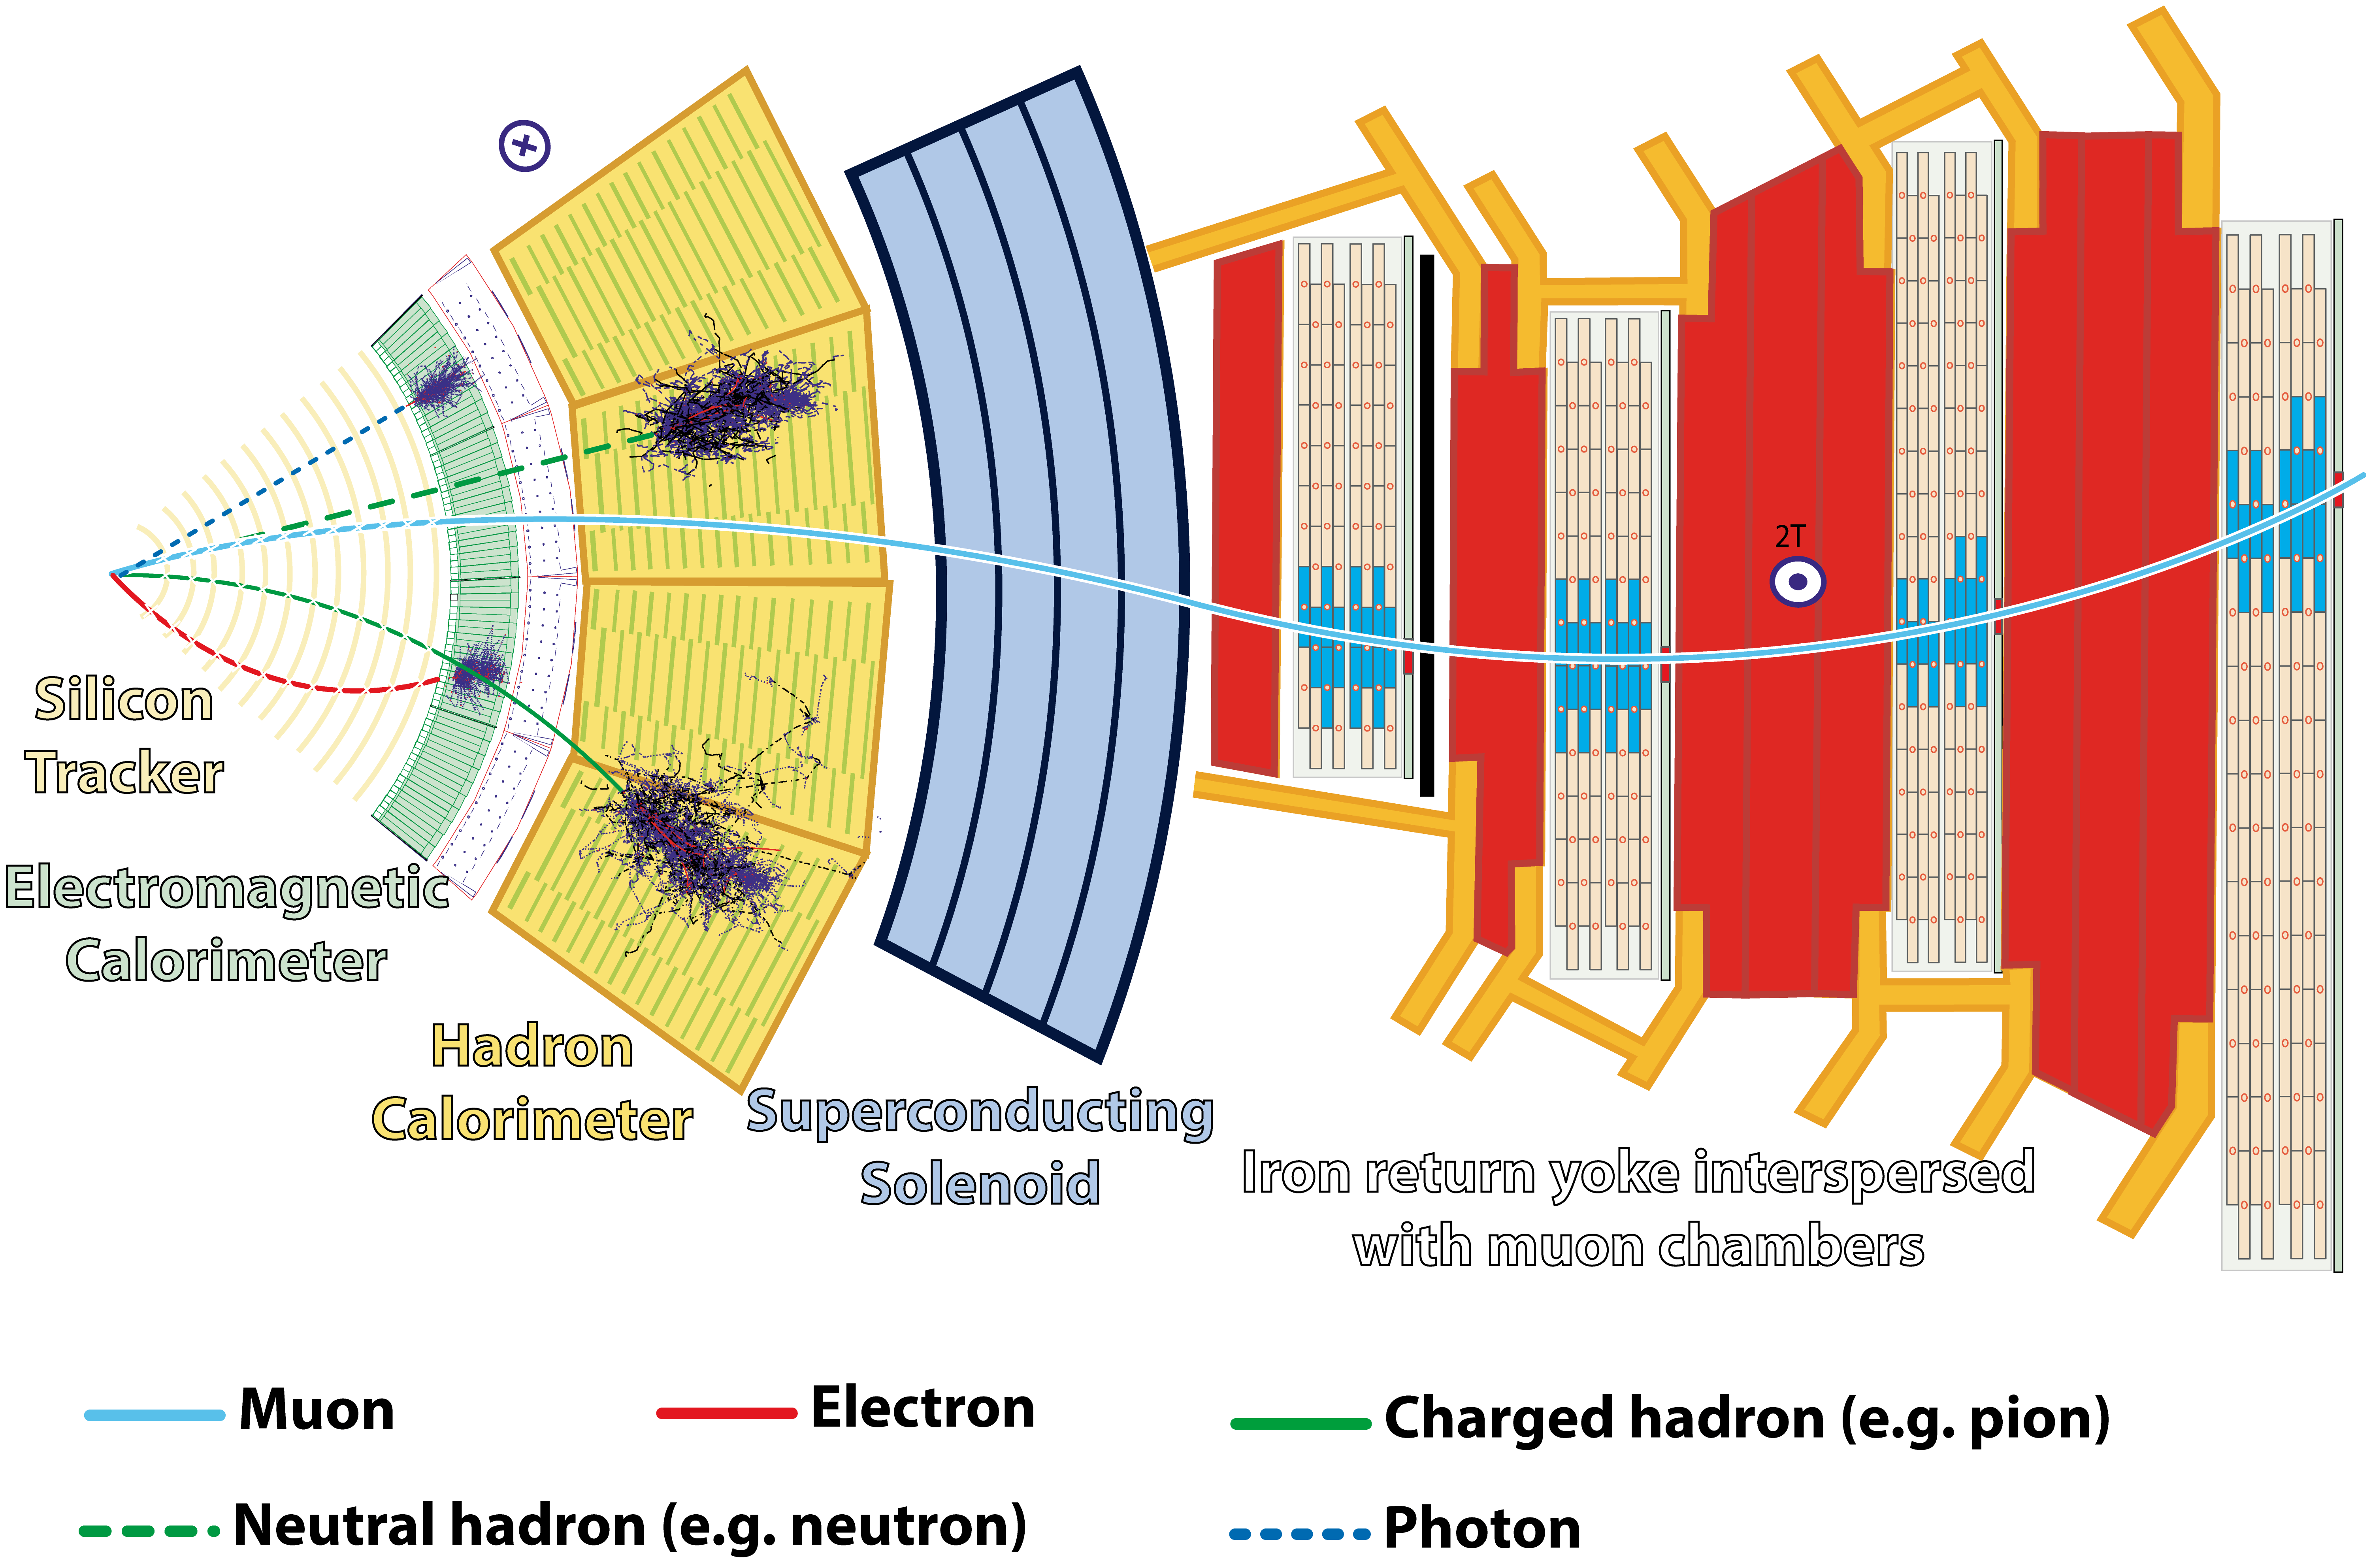
\includegraphics[width=.75\linewidth]{fig/CMS_Slice.png}
\end{center}
\caption{A section slice of the CMS detector where we can see how 
particles with different physical properties interact differently with the detector.\protect\footnotemark}
\label{fig:CMS_Slice}
\end{figure}
\footnotetext{\url{https://cds.cern.ch/record/2120661}}

One important kind of `final-state' particles used in this thesis is charged lepton, 
which includes electrons and muons (the half-life of tau-on is too short to interact with
the detector directly);
`final-state' here means they are the end products of a decay chain and are recorded by the detector
components directly. If we concentrate on the red and blue lines in Fig.~\ref{fig:CMS_Slice}, we
can see that electrons (red) leave a few hits that resemble a curved
track within the silicon tracker and are stopped at the electromagnetic calorimeter
(ECAL). 

For the muons (blue line in Fig.~\ref{fig:CMS_Slice}), they largely go through all the interior layers unhinged 
due to their higher mass and the fact that they only interact electromagnetically (unlike a proton, for example);
pay close attention to the `S'-shaped curve, this is due to the opposite magnetic
field outside of the superconducting solenoid. The iron return yoke also stops particles other than
muons coming through (except neutrinos which always travel freely). Although information such as momentum relies on
hits on the silicon trackers, the hits in the muon chambers and a matching trajectory are needed 
for the object to be reconstructed as a muon. Notice how the
muon chambers occupy more than half of the detector by size. Such a design allows the CMS 
detector to excel in muon measurements and is the primary reason for the overall design.
% \todo[inline]{TODO: PF and anti-k algorithm in the context of this thesis}

Zooming out from the individual components of the detector, the complete (physics object) reconstruction
process is complex and sometimes requires information from multiple parts of the detector. This
algorithm is called the Particle Flow (PF)~\cite{particle_flow}. While the energy of simple and neutral 
objects such as photon are directly measured by the ECAL (with correction such as zero-suppression, where minimal
activities are treated as zero value during readout), electron measurements
need the information from the inner tracker (to determine charge and momentum), energy at the ECAL, and
also, the sum of the energy of photons produced by bremsstrahlung (when electron interacts with the 
detector material) compatible with the electron's track.

For gluons and quarks that come out of the interaction vertex, due to quark confinement, the detector 
is only be able to `see' a narrow `spray' of final state (stable) particles that subsequently
are clustered into objects called `jets'.
There are different algorithms and criteria to combine a collection of measurements into a single jet,
in the CMS at the moment, the anti-$k_t$ clustering algorithm~\cite{anti_k,fastjet} is used. In short, the algorithm would cluster objects
in a roughly cone-like space that originated from the vertex according to some parameters.
The algorithm is resilient to QCD effects that would cause jets to split, such as shown in Fig.
\ref{fig:jet_split}

\begin{figure}[htb]
\begin{center}
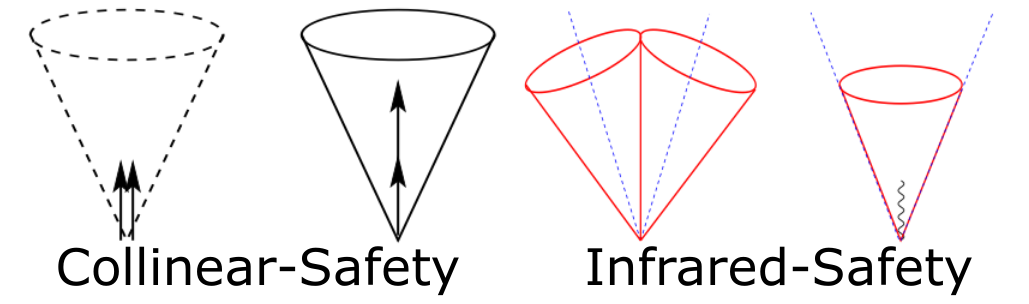
\includegraphics[width=.85\linewidth]{fig/jet_split.png}
\end{center}
\caption{A illustration of two kinds of QCD effects in jets\protect\footnotemark}
\label{fig:jet_split}
\end{figure}
\footnotetext{\url{https://twiki.cern.ch/twiki/bin/viewfile/Sandbox/Lecture?rev=1;filename=Philipp\_Schieferdeckers\_Lecture.pdf\#page=3}}

In this analysis, we use the AK4 jets which means that the algorithm is given a $R=0.4$ parameter. Another
common choice is $R=0.8$, which is preferred in some cases for boosted topologies due to a larger `opening
angle'.

\section{The Higgs boson and off-shell methods}\label{sec:physics_offshell}
% [1]Caola F, Melnikov K. Constraining the Higgs boson width with ZZ production at the LHC. Phys Rev D 2013;88:054024. https://doi.org/10.1103/PhysRevD.88.054024.


As mentioned above, the Higgs boson has a special place as it can be seen as a `bridge' between
the SM and the BSM (in some models), as some SUSY particles can decay into it or decay out from it, 
or simply have a BSM production Feynman diagram that leads to a higher Higgs
bosons production rate than the SM expects. In any of these cases, the basic properties of the SM Higgs
boson remains important.

The importance of studying the Higgs also comes from the fact that it is an `add-on' to the SM as
a mass generation mechanism for gauge bosons and fundamental fermions. The Higgs sector of the SM is not well tested, 
and, in theory, could be more complicated than the minimal SM suggests. For example, multiple Higgs bosons
may be present,
or the observed Higgs may be a composite particle. Interestingly, if not composite, the observed Higgs boson would be the only
spin-zero fundamental particle we know.


Many properties are well measured, such as its mass and spin~\cite{cms_higgs}; others, however,
have not entered the realm of `precision' physics so far. One of them is the total decay width of
the Higgs boson, which is of course associated with the particle's half-life $\tau$ as $\Gamma=\frac{\hbar}{\tau}$.
The SM predicts
that the Higgs boson will have a decay width of \SI{4.07}{\mega\electronvolt}. The problem is
that the energy resolution of the CMS detector, which is around $\mathcal{O}(1) $\si{\giga\electronvolt}
for the di-photon or 4-leptons final states, is not even remotely close to that prediction.

One way to measure the decay width suggested by the theorists is to indirectly measure it using the
off-shell method~\cite{offshell_theory1, offshell_theory2}. When a Higgs boson decays into two massive
vector bosons (VV) (in the scope of this thesis, two Z bosons),
one of them has to be off-shell, or the Higgs boson is off-shell. This is because
$m_\text{H}\approx\SI{125}{\giga\electronvolt}$ is smaller than the 
mass of two W-bosons ($\approx\SI{160}{\giga\electronvolt}$) 
or of two Z-bosons ($\approx\SI{182}{\giga\electronvolt}$). The Higgs boson decay branching ratio
is coupled to the daughter particles' mass, and thus this cross-section
$\sigma_{\mathrm{H}\rightarrow\mathrm{VV}}$ is enhanced as the mass of Higgs boson gets closer to 
the on-shell VV mass.  

In fact, the production of Higgs boson from a pair of vector boson is also related to the
decay width of Higgs boson $\Gamma_\text{\PH}$ via the `propagator'\cite{offshell_poc}. In terms of the
differential cross-section:

\be
\label{eqn:diff_xsec}
\frac{\mathrm{d} \sigma_{\mathrm{vv} \rightarrow \mathrm{H} \rightarrow \mathrm{VV}}}{\mathrm{d} q_{\mathrm{H}}^{2}} 
\sim 
\frac{g_{\mathrm{vvH}}^{2} g_{\mathrm{HVV}}^{2}}{\left(q_{\mathrm{H}}^{2}-m_{\mathrm{H}}^{2}\right)^{2}+m_{\mathrm{H}}^{2} \Gamma_{\mathrm{H}}^{2}}
\ee

where the two $g$ on the right-hand side are the couplings for production from vv and decay
to VV respectively. By integrating this equation near the on-shell mass of the SM Higgs boson 
or in the tail region (above the mass of a pair of V's), one can translate the differential cross section
into event rate that can be (in theory) measured in experiments:
\begin{equation}
\begin{split}
&N_{\mathrm{vv} \rightarrow \mathrm{H} \rightarrow \mathrm{VV}^{*}}^{\text{on-shell}} \sim \frac{g_{\mathrm{vvH}}^{2} g_{\mathrm{HVV}}^{2}}{m_{\mathrm{H}} \Gamma_{\mathrm{H}}} \sim \mu_{\mathrm{vvH}}
\\
&N_{\mathrm{vv} \rightarrow \mathrm{H}^{*} \rightarrow \mathrm{VV}}^{\text{off-shell}} \sim \frac{g_{\mathrm{vvH}}^{2} g_{\mathrm{HVV}}^{2}}{\left(q_{\mathrm{H}}^{2}-m_{\mathrm{H}}^{2}\right)^{2}} \sim \mu_{\mathrm{vvH}} \cdot \Gamma_{\mathrm{H}}
\end{split}
\end{equation}
The key takeaway is that, up to some correction factors, the event rate of off-shell Higgs scales
linearly respect to the Higgs decay width $\Gamma_\text{\PH}$ which allows indirect
measurement of the width itself.

In this thesis, we will focus on the $\mathrm{H} \rightarrow \mathrm{ZZ} \rightarrow 2\ell2\nu$ channel
at the CMS detector using simulated (MC) events. The work conducted here is part of the ongoing analysis
within a group formed by the UCSB HEP group, Universit\'e Libre de Bruxelles, and Beihang University under
the CMS Collaboration\footnote{Internally, CMS AN-20-081}. The analysis items and methods included in this
thesis are a subset of what will be in the official analysis and is a part of the final measurement. More
details on what approximations have been taken in order to obtain a preliminary expected result will be discussed
in the next few sections.

% \todo[inline]{maybe elaborate a bit more?}
% \newpage\phantom{blabla}


\section{Background and signal simulation}
% [1]Agostinelli S, Allison J, Amako K, Apostolakis J, Araujo H, Arce P, et al. Geant4—a simulation toolkit. Nuclear Instruments and Methods in Physics Research Section A: Accelerators, Spectrometers, Detectors and Associated Equipment 2003;506:250–303. https://doi.org/10.1016/S0168-9002(03)01368-8.

% [2]Gritsan AV, Roskes J, Sarica U, Schulze M, Xiao M, Zhou Y. New features in the JHU generator framework. ArXiv:200209888 [Hep-Ex, Physics:Hep-Ph] 2020.

% [3]The NNPDF Collaboration, Ball RD, Bertone V, Carrazza S, Deans CS, Del Debbio L, et al. Parton distributions for the LHC Run II. J High Energ Phys 2015;2015:40. https://doi.org/10.1007/JHEP04(2015)040.

% [4]Melia T, Nason P, Röntsch R, Zanderighi G. W+W-, WZ and ZZ production in the POWHEG BOX. J High Energ Phys 2011;2011:78. https://doi.org/10.1007/JHEP11(2011)078.

% ---
The following list contains the MC samples (by physical process) used in this thesis, the first two
contain (off-shell) Higgs boson in the intermediate state:
\begin{itemize}
\item ggZZ offshell: Gluon fusion $\textsl{g}\textsl{g} \rightarrow\mathrm{H}\rightarrow\mathrm{ZZ}$
\item VVZZ offshell: Vector boson fusion (VBF) into Higgs boson
\item qqZZ, qqWZ, qqWW
\item DY: Drell-Yan process
\item TT: $t\bar{t}$, including samples with additional vector boson (TTW/TTZ) or photon + jets (TTGJets).
\end{itemize}

The MC samples for all processes except DY are produced in Run 2 Autumn18MiniAOD-102X analysis,
DY sample is produced in Run 2 Summer16MiniAODv3 94X analysis and scaled appropriately afterward. As their names
suggest, each year in the Run 2 (2016-2018) has their separate MC samples since the running condition
(the LHC) and the condition of CMS can change from year to year, though the physics remains the same.

Various programs are used in the long chain of simulated events production.
\textsc{POWHEG v2}\xspace\cite{powhegv2}, \textsc{JHU generator and MELA}\xspace\cite{jhugen}, are used for 
the signal simulation.
\textsc{MadGraph}\xspace\cite{madgraph} is used to generated NLO background samples, 
\textsc{Pythia}\xspace\cite{pythia} for parton
showering and \textsc{NNPDF} 3.1\cite{nnpdf} sets are used for the parton distribution functions.
% \todo[inline]{A description of LO / NLO and various program and NNPDF version etc.\ involved}

Before diving into the procedure in which the signal samples are generated separately and
subsequently combined via a reweighting, it would be appropriate to give
an account for the general idea behind the `event weight' and its significance.

As described at the beginning of this section, events that correspond to different physical
processes are generated in different MC configurations at different `orders' of the QCD/QED physics.
Naively, one would imagine a process where the MC can directly simulate the complete physics at
the LHC at a given center-of-mass energy. Unfortunately, this is neither efficient nor possible.
It is not possible because some physical processes (especially QCD ones) are non-perturbative and
stepped approaches are taken to gradually build-up to the final event.
It is also impossibly inefficient because the processes that an analysis is concerned with 
(for example, in all SUSY searches) usually have a tiny (if not 0)
cross-section compared to other common processes that can be
found at
$\sqrt{\mathrm{s}} = \SI{13}{\tera\electronvolt}$ at the LHC.\@ And it would be a waste of
computing resources to generate common processes over and over again.

\begin{table}[ht]
\centering
\begin{tabular}{|c|c|c|}
\hline
\multicolumn{3}{|c|}{Example of some important weights}                                                                                       \\ \hline
Name                  & abbr.   & Description                                                                                                 \\ \hline
Generator weight      & GEN wgt & Given by MC event generator                                                                                 \\ \hline
Pile-up weight        & PU wgt  & Correction for the pile-up effect\footnotemark                                                                           \\ \hline
Matrix element weight & ME wgt  & From generator that uses ME Likelihood approach \\ \hline
K-factor              & Kfactor & Correction for LO cross section of QCD processes                                                         \\ \hline
\end{tabular}
\caption{An incomplete list of weights used in the MC events used.}
\label{tab:MC_wgts}
\end{table}

In reality, Monte Carlo events are each given many `weights' (Tab. \ref{tab:MC_wgts}), so that
we don't have to generate uninteresting processes. At the same time, for the events that lack
in number (i.e.\ it results in poor statistical distribution), one can optionally generate
extension events set for it. In practice, (for example as shown in Fig.~\ref{fig:wgt_demo})
you can have \num{1e6} raw MC entries, but only
100 expected events (yield) in the integration of the histogram, 
due to the physics process being very rarely seen. But,
these \num{1e6} would form a much smoother distribution than if you only had 100 entries to work with.
Also, this enables the generation of `unknown' processes which can
be used to constrain possible new physics in a likelihood fit (against null hypothesis).
\footnotetext{when many unwanted collisions happen in the same bunch crossing}

\begin{figure}[hb]
\begin{center}
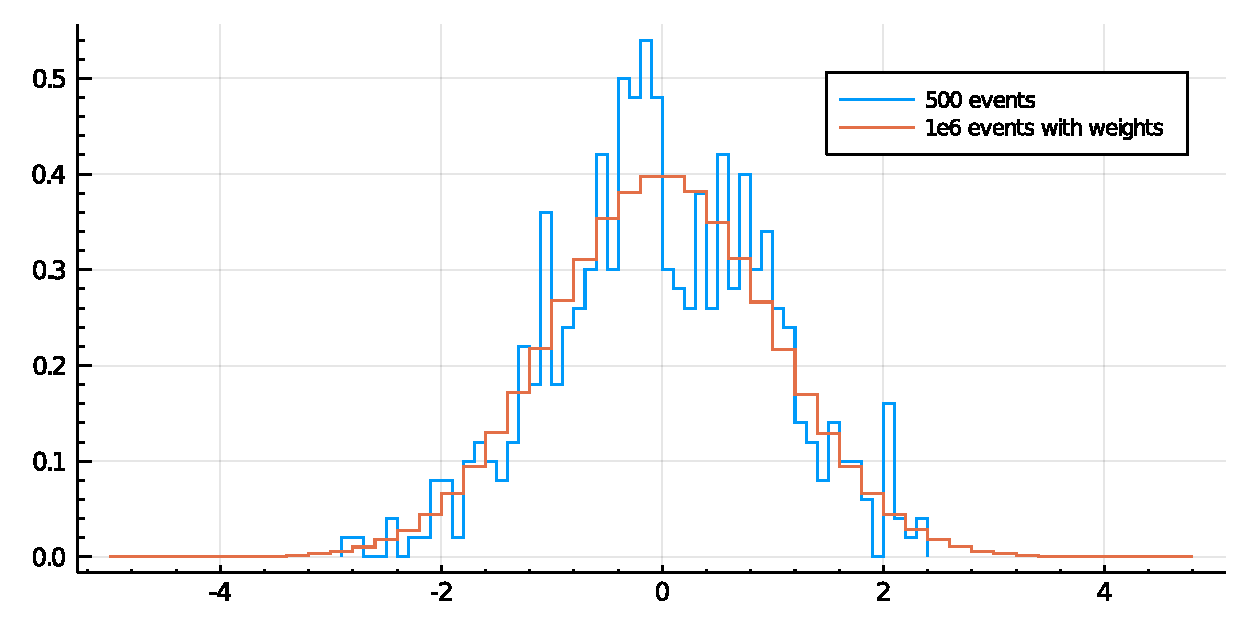
\includegraphics[width=.8\linewidth]{fig/demo_wgts.pdf}
\end{center}
\caption{Illustrative plot to show how weights can make distribution smoother without altering
the total number of expected events.}
\label{fig:wgt_demo}
\end{figure}

In this thesis, we explicitly use K-factors, and variations of it to 
obtain Electroweak systematical uncertainty in qqZZ/qqWZ/qqWW backgrounds. For the signal processes involving
the Higgs boson, special treatment is given to merging and obtaining high-statistics samples from
multiple `raw' samples with different pole mass of Higgs boson corresponding to the $m_\mathrm{H}$ term
in the denominator on the right-hand side of Eq.~\ref{eqn:diff_xsec}.
This approach is also desirable for the generation of off-shell (Higgs) decays. The procedures 
used and the resultant combined signal samples are discussed in the Sec.~\ref{sec:sig_rewgt}.

\section{Uncertainties}
A limited number of experimental and theoretical uncertainties in both signal and background
processes are discussed here. Although dedicated to MC-only analysis, the leading theoretical
uncertainties are considered:
\begin{table}[hbt]
    \label{tab:uncertainty}
    \centering
\begin{tabular}{lcc}
\hline
Source                             & Uncertainty            & Affected processes \\ \hline
Integrated luminosity              & 2.5\%                  & ggZZ, VVZZ, qqZZ, qqWZ \\
Non-resonant background estimation & 10\%                   & TT, qqWW           \\
Electroweak                       & 1$\sigma$ & qqZZ, qqWZ         \\
Higgs branching ratio              & 2\%                    & ggZZ, VVZZ           \\
gg background              & 10\%                   & ggZZ
\end{tabular}
\caption{Summary of systematic uncertainties considered in this thesis and their
magnitude as well as processes affected by them.}
\label{tab:systs}
\end{table}

Most of the uncertainties are simply experimental, for example, the luminosity. The Electroweak (EW)
uncertainties are obtained by scaling EW NLO K-factor up or down on the corresponding samples and non-resonant
background comes from separate studies that examine $e/\mu$ events in the data, which
are limited by the number of events within the Z-boson mass window. Here we approximate this 
uncertainty as $\pm 10\%$.  The gg background uncertainty is parametric respect to the $\mtzz$ defined 
below~\cite{campbell_two_2016, caola_qcd_2015, caola_qcd_2015}.

